\section{Evaluation} \label{sec:Evaluation}

In this section we explain how we evaluate the feasibility of automated transplantation in video games through our \ApproachName{} approach. To do so, we have run an experiment evaluating our approach, \ApproachName, with a measure from the literature, and we have conducted a preliminary evaluation with human developers.
Through this section, we will present the research questions that we aim to answer, the evaluation
process (including the measure quality for the solutions and baseline), and the implementation details.

\subsection{Research Questions}
We aim to answer the following research questions:
\RQ{What is the quality of the models generated by
Imhotep in contrast to the models from the oracle?}
\RQ{What is the quality of the models generated whith each variant of Imhotep (Simulation and Test-based)?}
\RQ{Is there significant difference between a traditional PCG approach and a transplantation approach?}

\subsection{Planning and execution}

Figure~\ref{fig:evaluation} shows an overview of the evaluation process. The upper part of the figure shows the software models selected from the original video game content provided by developers from \CaseStudy{}, which are the inputs for the test cases. 

In the figure, the output of the test cases are a baseline and the two variants of our approach. We used the work by Gallota \etal~\cite{gallotta2022evolving} as PCG baseline. Gallota \etal presented a hybrid Evolutionary Algorithm for generating NPCs, more precisely spaceships. Their approach combine an L-system with Feasible Infeasible Two Population Algorithm. Gallota \etal were able to evolve spaceships that match some statistics of human-designed spaceships.
The two variants of our \ApproachName{} approach work as
described in Section~\ref{sec:Approach} to form the transplanted models that are considered to be the most relevant transplantations.

The evaluate the output of the test cases we compare them with an oracle. The oracle is extracted from the original software models from the video game \CaseStudy{}. The oracle and the output pass through a simulation provided by the game developers of \CaseStudy{}, which simulates an in game battle between the boss and a player. From the simulation we extract the duration, which is a metric used by the literature~\cite{browne2010evolutionary}.

{\bf Duration:} The duration of duels between players and boss units is expected to be around a certain optimal value. For the video game case study, through tests and questionnaires with players, the developers determined that concentration and engagement for an average boss reach their peak at approximately 10 minutes ($T_{Optimal}$), whereas the maximum accepted time was estimated to be 20 minutes ($2*T_{Optimal}$). Significant deviations from that reference value are good design-flaw indicators: short games are probably too easy; and duels that go on a lot longer than expected tend to make players lose interest. The criterion $Q_{Duration}$ is a measure of the average difference between the duration of each duel ($T_{d}$) and the desired, optimal duration ($T_{Optimal}$):
\begin{equation}
Q_{Duration} =  1 - \frac{\sum\limits_{d=1}^{Duels}\frac{\mid T_{Optimal} - T_{d} \mid}{T_{Optimal}}}{Duels} 
\end{equation}

\begin{figure}[h]
    \centering
    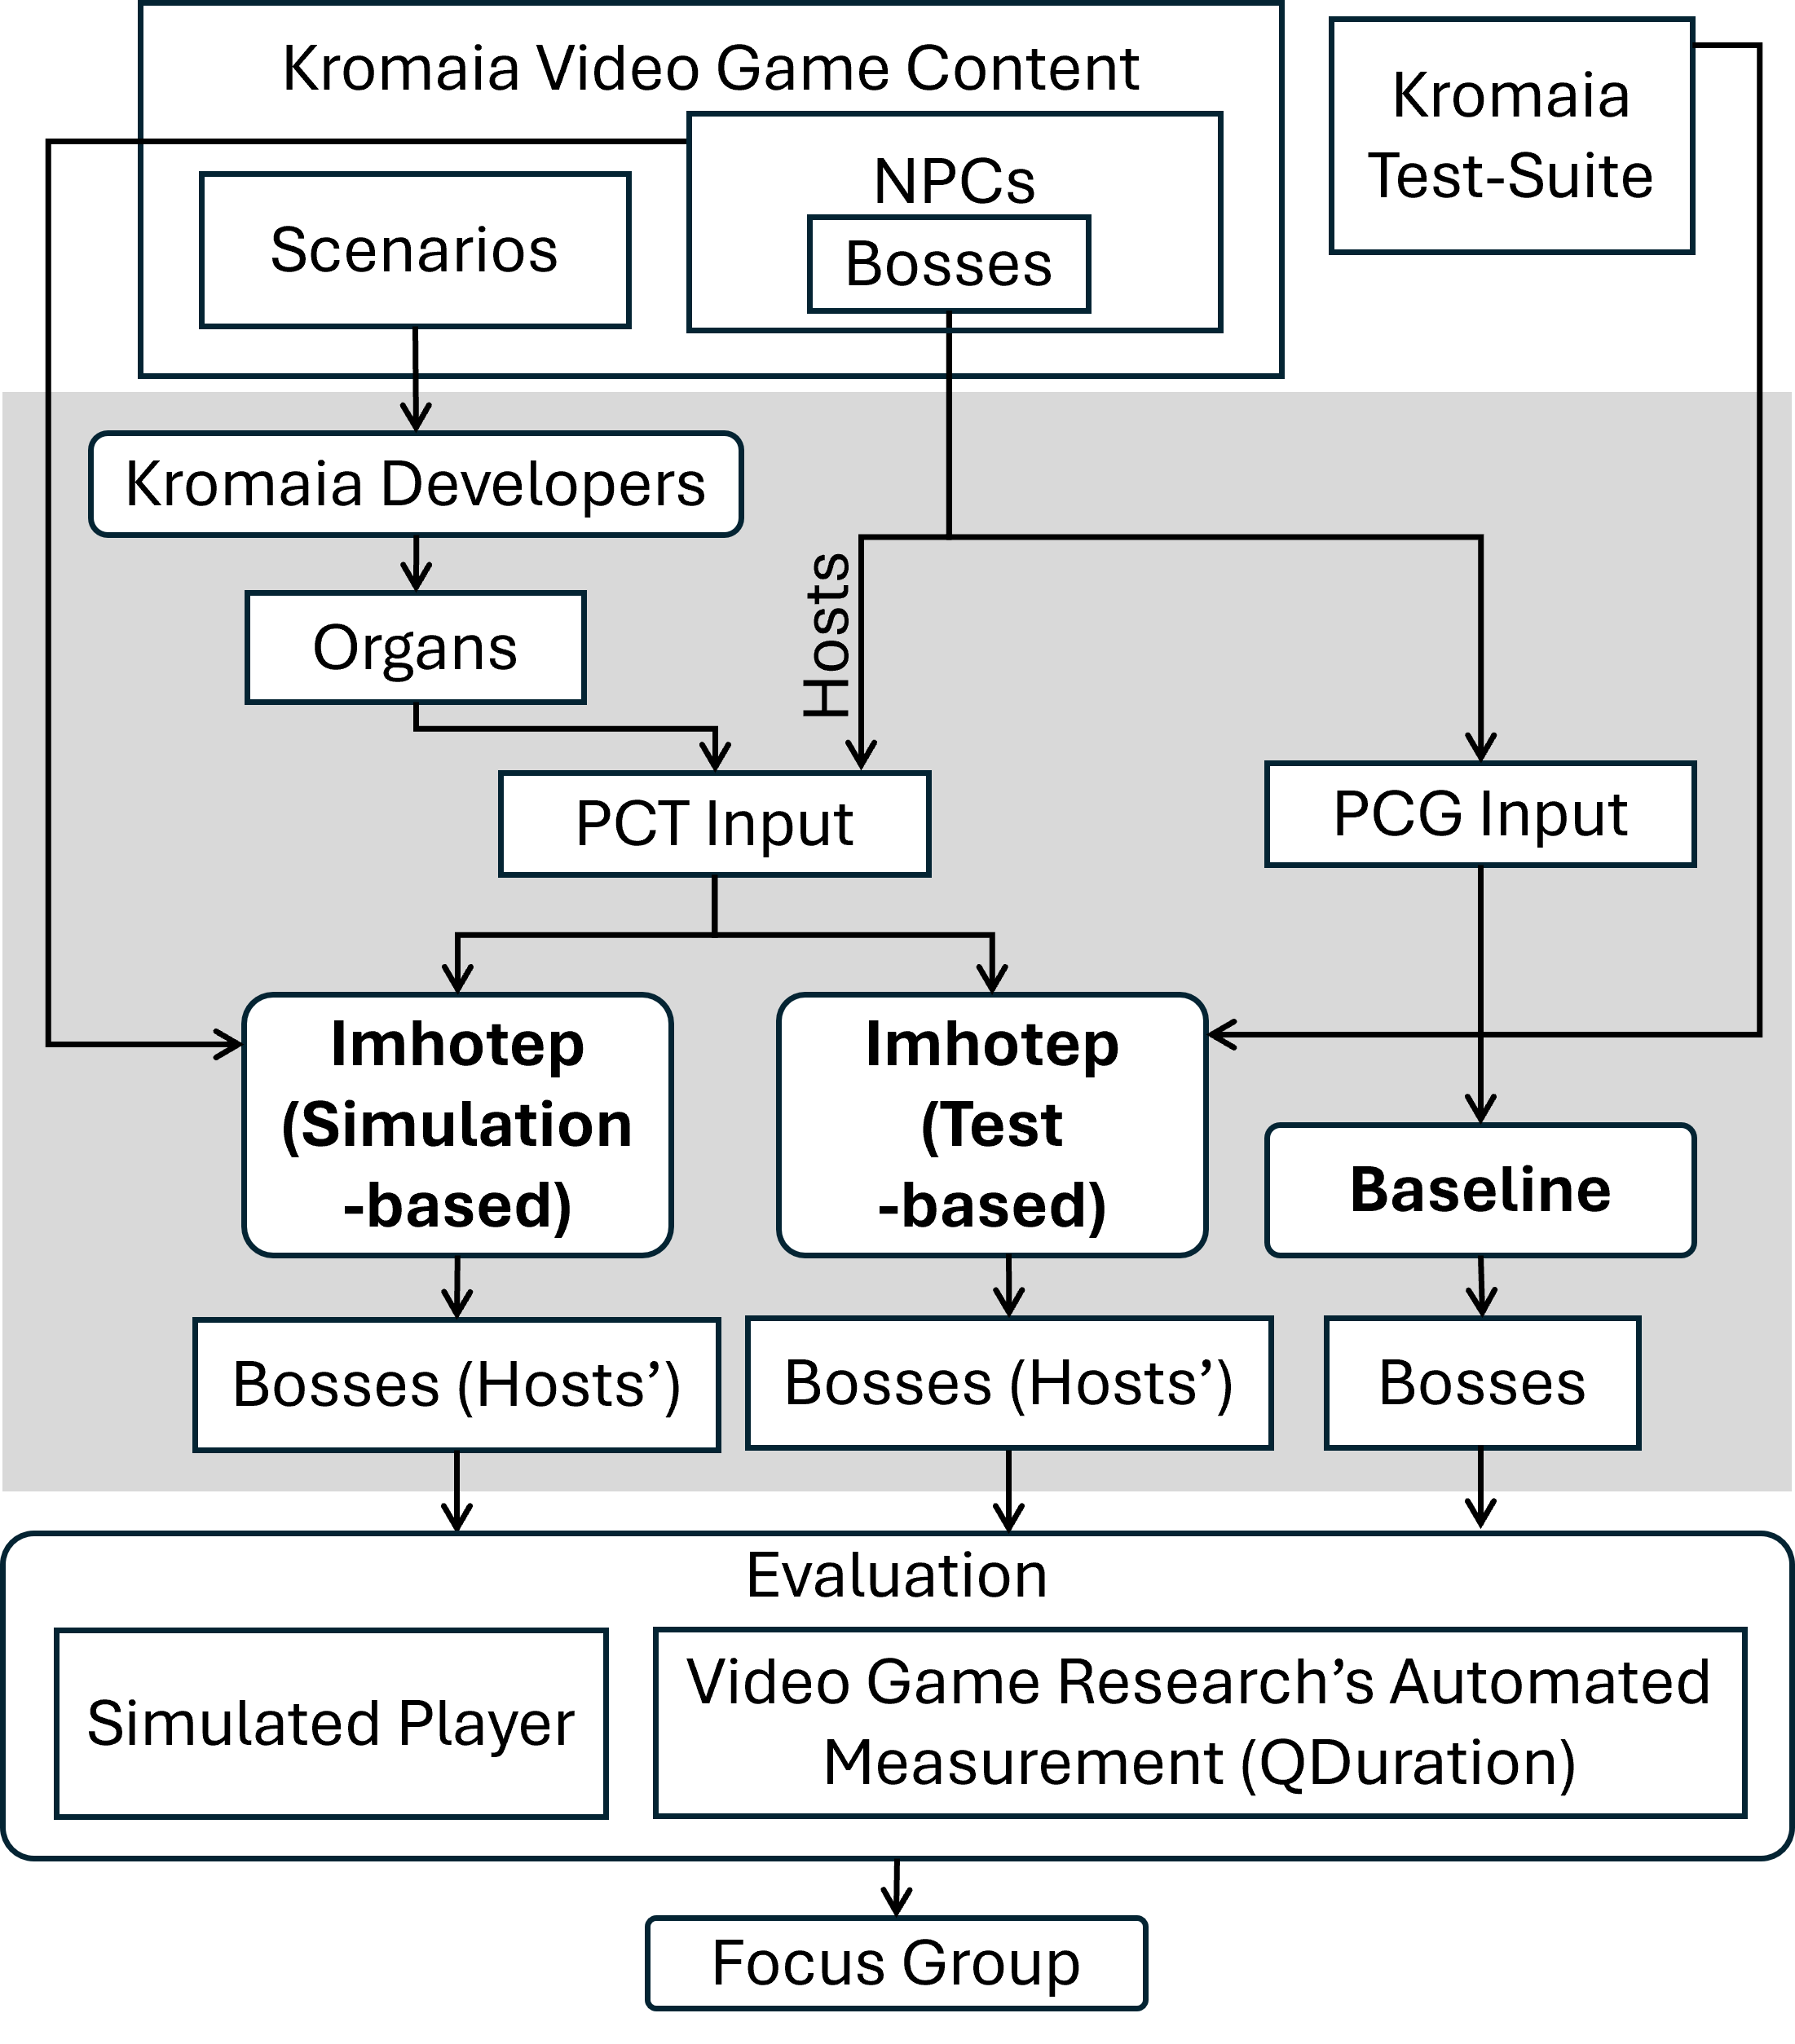
\includegraphics[width=0.45\textwidth]{Figures/evaluation_process.png}
    \caption{Overview of our evaluation process.}
    \label{fig:evaluation}
\end{figure}

\subsection{Implementation details}

For the evaluation we used 5 different host (Vermis, Teuthus, Argos, Orion, and Maia), which are original bosses from the video game \CaseStudy{}. As a donor we used the scenario of the video game, and we collected 129 organs, that are elements from the scenario. Each organ was transplanted individually to each boss. Hence, we obtain a total of 645 new individuals (5*129). Each variant of \ApproachName{} provided a total of 645 new individuals as output, 645 new individuals from Simulation-based and 645 individuals from Test-based. In the case of the baseline, to make it fair, the approach was executed 129 times with each one of the 5 different hosts to obtain 645 new individuals.

In order to compare the baseline and variants of our approach, we chose the parameters shown in Table~\ref{tab:evaluation_parameters} to calibrate the evolutionary algorithm and the objective function. We established the stop condition at 2 minutes and 30 seconds, ensuring that the approaches run long enough to obtain the best solutions. Even though the population size is 100 individuals, we only present to the best of the variants and in the baseline. We assume that the best candidate solutions are those with the highest objective function value.

The evaluation of \ApproachName{} and the baseline was done
using two Pcs with the following specifications; Intel Core i7-8750H, 16GB, 2.2GHz; and  2x Intel(R) Xeon(R) CPU X5660, 64GB, 2.80GHz.
The implementation uses the Java(TM) SE Runtime Environment (build 17.0.5), together with Java as the programming language. 
For purposes of replicability, the implementation source code and the data (software models and oracles) are publicly available at the following URL:


\mar{Need to confirm the Java version, and ask for the data for replicability. I have only the CSVs of the results.}

\begin{table}[h]
    \centering
    \begin{tabular}{ll}
        \hline
        \bf{Parameter description}            & \bf{Value}  \\ \hline
        Stop Time                        & 2m 30s \\
        Population Size                  & 100    \\
        Number of parents                & 2      \\
        Number of offspring from parents & 2      \\
        Crossover probability            & 1      \\
        Mutation probability             & 1/150 \\ \hline
    \end{tabular}
    \caption{Parameter settings}
    \label{tab:evaluation_parameters}
    \end{table}

% \subsection{Quality measurements}
% \label{subsec:Measurements}

% In a recent research done by Browne et al., the experimentation with game users showed that the following criteria stand out as being the most important: Completion, Duration, Uncertainty, Killer Moves, Permanence, and Lead Change \cite{browne2010evolutionary}. Our evaluation measures these criteria with values in the interval [0,1].

% {\bf Completion (Viability):} A game against a boss unit should end with more conclusions (victories for either the player or the boss) than draws/ties. The criterion $Q_{Completion}$ calculates a ratio of conclusions over total duel count:
% \begin{equation}
% Q_{Completion} = \frac{Conclusions}{Duels}
% \end{equation}

%  {\bf Uncertainty (Quality):} In order to keep players engaged with a duel, neither the player nor the boss unit should get extremely close to victory or defeat too early before the duel is settled, with ($T_{d}$) being its duration. Therefore, a duel is considered to be more uncertain the longer the time until the player's or the boss unit's health levels reach a dangerous/critical status ($P_{d}$ and $B_{d}$, respectively). For each duel, $Q_{Uncertainty}$ measures the average deviation between the time at which it is detected that one of the contenders is on the verge of defeat and the time corresponding to the duration of the duel.
% \begin{equation}
% Q_{Uncertainty} =  1 - \frac{\sum\limits_{d=1}^{Duels}\frac{T_{d} - min\left ( P_{d}, B_{d} \right )}{T_{d}}}{Duels} 
% \end{equation}

% {\bf Killer Moves:}   $Q_{KMoves}$ measures the proportion of killer moves by any contender ($K$), taking into account the moves that are considered to be remarkable highlights ($H$) but that are less important than killer moves. In the video game case study, the developers considered that a highlight move happens when either the boss unit or the player experiences a decrease in health; killer moves are those that make the difference in health between the contenders reach 30\%.
% \begin{equation}
% Q_{KMoves} =  1 - \frac{\sum\limits_{d=1}^{Duels}\frac{K_{d}}{H_{d}}}{Duels} 
% \end{equation}

% {\bf Permanence:} Duels with a high permanence value are games in which the advantages given by significant actions or moves by one of the contenders are unlikely to be immediately reverted by the opponent in terms of dominance. In the video game case study, the developers considered every highlight move and killer move to be meaningful actions, with recovery moves ($R$) being those that quickly cancelled the advantages given by other previous killer or highlight moves. The criterion $Q_{Permanence}$ is measured as follows:
% \begin{equation}
% Q_{Permanence} =  1 - \frac{\sum\limits_{d=1}^{Duels}\frac{R_{d}}{H_{d}+K_{d}}}{Duels} 
% \end{equation}

% {\bf Lead Change:} The lack of lead changes indicates low dramatic value. In the video game case study, the lead is determined at any given moment by considering the contender with the highest health level. This criterion is measured taking into account those highlight or killer moves that cause the lead to change ($L$) during the course of a duel:
% \begin{equation}
% Q_{LChange} = \frac{\sum\limits_{d=1}^{Duels}\frac{L_{d}}{H_{d}+K_{d}}}{Duels} 
% \end{equation}

% $Q_{Overall}$ calculates an average quality value for a model, including all of the quality criterion studied:
% \begin{equation}
% Q_{Overall} = \frac{\sum\limits_{i=1}^{N}Q_{i}}{N}
% \end{equation}